\section{Recherche de solution}

\subsection{L'algorithme de Canny}

\subsubsection{Version de base}
Le filtre de Canny a été créé en 1986 dans le but d'améliorer les résultat du filtre de Sobel.
Le principe du filtre est d'utiliser deux filtres, un filtre haut et un filtre bas. L'algorithme
commence par séléctionner les pixels supérieur au seuil haut, puis recherche à partir de chaque
pixels au dessus du seuil haut les pixels qui sont au dessus du seuil bas. Ainsi on voit 
que cet algorithme prend en compte deux caractèristiques, l'intensité et la direction des 
gradients.\\

Nous utilisons cette algorithme dans les régions autour des yeux afin de délimiter le contour
de chaque oeil. Le résultat permet de faire ressortir l'oeil mais aussi les sourcils et certaines
ombres présentent dans le creu de l'oeil. Ce filtre permet donc de détecter les contours des yeux,
mais le résultat comporte beaucoup de bruit. 

\begin{figure}[H]
 \center
 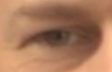
\includegraphics[width=4cm]{image/original.png}
 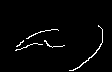
\includegraphics[width=4cm]{image/canny_moyenne.png}
 \caption{Image de test et résultat de l'algorithme de Canny avec une moyenne des pixels}
\end{figure}

Peu efficace -> recherche d'une meilleur détermination des seuil de Canny

\subsubsection{Avec une moyenne de pixels sur des parties d'image}

décomposition de l'image en plusieurs sous images
\begin{figure}[H]
 \center
 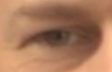
\includegraphics[width=4cm]{image/original.png}
 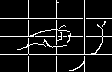
\includegraphics[width=4cm]{image/canny_decomposition.png}
 \caption{Image de test et résultat de l'algorithme de Canny avec division de l'image en 16}
\end{figure}

problème trait et bruit

\subsubsection{Erosion et dilatation des sous-images}

objectif -> supprimer les traits + suppression du bruit (ombre + ride)
\begin{figure}[H]
 \center
 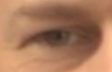
\includegraphics[width=4cm]{image/original.png}
 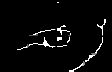
\includegraphics[width=4cm]{image/canny_final.png}
 \caption{Image de test et résultat de l'algorithme de Canny avec dilatation puis érosion des sous-images}
\end{figure}

\subsubsection{Avec égalisation d'histogramme}
% L'égalisation d'histogramme est un procédé qui essaye de placer le même nombre de pixels
% sur chaque composante de gris. Ce qui a pour effet d'augmenter le contraste de l'image
% et devrait ainsi améliorer les hautes fréquences de l'image, donc les contours. Nous avons
% essayé d'appliquer cette méthode sur une image en niveau de gris avant de lancer l'algorithme
% de Canny.
%TODO ajout des images

Quelque soit les traitements effectué au préalable sur l'image avant l'utilisation de l'algorithme de Canny
sur une image de gris, nous n'obtenons aucun résultat. Pour supprimer les ombres présentent sur les images
que nous traitons, nous décidons d'utiliser un autre modèle colorimètrique.

\subsection{Les modèles Colorimètrique}
\subsubsection{Le modèle HSV}

\begin{figure}[H]
 \center
 
\includegraphics[width=4cm]{image/hue.png}
 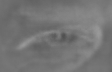
\includegraphics[width=4cm]{image/saturation.png}
 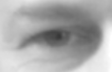
\includegraphics[width=4cm]{image/value.png}
 \caption{Décomposition du modèle HSV}
\end{figure}

solution -> calcul d'un masque avec la value pour réduire l'image pris en compte par canny

saturation -> probleme sur la couleur de peau.

\begin{figure}[H]
 \center
 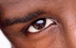
\includegraphics[width=4cm]{image/original_black.png}
 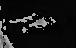
\includegraphics[width=4cm]{image/hue_black.png}
 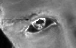
\includegraphics[width=4cm]{image/saturation_black.png}
 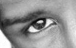
\includegraphics[width=4cm]{image/value_black.png}
 \caption{Décomposition du modèle HSV avec une couleur de peau plus foncée}
\end{figure}

\subsubsection{Le modèle YUV}

calcule RGB vers YUV
$$Y = 0.299R + 0.587 G + 0.114 B$$
$$U = -0.147R - 0.289 G + 0.436B = 0.492(B - Y)$$
$$V = 0.615R -0.515G -0.100B = 0.877(R-Y)$$

\begin{figure}[H]
 \center
 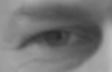
\includegraphics[width=4cm]{image/luminance.png}
 
\includegraphics[width=4cm]{image/chrominance1.png}
 
\includegraphics[width=4cm]{image/chrominance2.png}
 \caption{Décomposition du modèle YUV}
\end{figure}

\begin{figure}[H]
 \center
 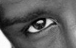
\includegraphics[width=4cm]{image/luminance_black.png}
 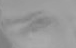
\includegraphics[width=4cm]{image/chrominance1_black.png}
 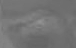
\includegraphics[width=4cm]{image/chrominance2_black.png}
 \caption{Décomposition du modèle YUV avec une couleur de peau plus foncée}
\end{figure}

\subsection{Détection des contours et calcul du barycentre de la forme}

\subsection{L'algorithme de Gabor}